\chapter{UML}

\begin{figure}[H]
    \centering
        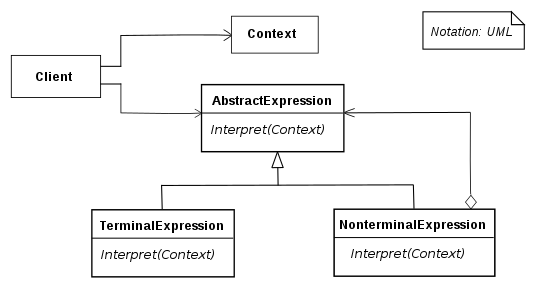
\includegraphics[width=0.8\textwidth]{figures/uml_class_diagram.png}
\end{figure}

These are the classes that are represented in the UML class diagram: 

\begin{itemize}
    \item \textit{AbstractExpression}: Declares an interpret() operation that all nodes (terminal and nonterminal) in the AST override.
    \item \textit{TerminalExpression} (\textit{NumberExpression}): Implements the interpret() operation for terminal expressions
    \item \textit{NonTerminalExpression} (\textit{PlusExpression, MinusExpression, DivideExpression, MultiplyExpression}): Implements the interpret() operation for all nonterminal expressions.
    \item \textit{Context(String)}: Contains information that is global to the interpreter. It contains the String expression with the Postfix notation that has to be interpreted and parsed.
    \item \textit{Client }: Builds the AST assembled from TerminalExpression and NonTerminalExpression. The Client invokes the interpret() operation.
\end{itemize}

The nonterminal symbols forward interpret the \textit{interpret} methods. This means, that you only need to call it once for the root node, because they will automatically call it on their list of child nodes. The \textit{TerminalExpression} cannot have any children. Only the \textit{NonTerminalExpression} can have one or more children. To see the interactions between the different object, look at the example in the next chapter.
